\documentclass[12pt,a4paper,oneside]{scrartcl}
\usepackage{blindtext}
\usepackage[T1]{fontenc}
\usepackage[utf8]{inputenc}
\usepackage{graphicx}
\usepackage{url}
\usepackage{float}
\usepackage[nodayofweek,level]{datetime}
\bibliographystyle{unsrt}

\setlength{\voffset}{-28.4mm}
\setlength{\hoffset}{-1in}
\setlength{\topmargin}{20mm}
\setlength{\oddsidemargin}{25mm}
\setlength{\evensidemargin}{25mm}
\setlength{\textwidth}{160mm}
\setlength{\parindent}{0pt}
\setlength{\textheight}{230mm}
\setlength{\footskip}{20mm}
\setlength{\headsep}{50pt}
\setlength{\headheight}{0pt}
\usepackage{hyperref}

\title{3D Beamforming for Matrix US probe}
\subtitle{Klinisches Anwendungprojekt}
%\author{Adrian Riedl}
\date{\formatdate{14}{10}{2019}}

\begin{document}

\maketitle

\section{Background}

The Chair for Computer Aided Medical Procedures published with SUPRA an open source pipeline for fully software defined ultrasound processing for real-time applications \cite{Goebl2018supra}.

Hence, SUPRA covers everything from beamforming to the output of B-mode images, running on consumer GPUs in real-time both in 2D and 3D.

\begin{figure}[h!]
\begin{center}
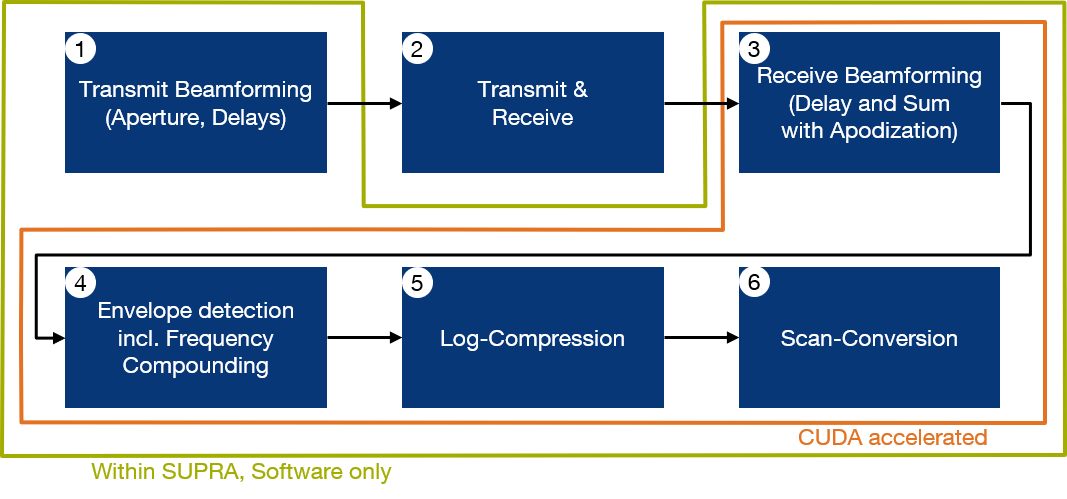
\includegraphics[width = \textwidth ]{Bilder/UsPipeline_color.png}
\caption[Pipeline of SUPRA]{Pipeline of SUPRA}
\label{Pipeline}
\end{center}
\end{figure}

Figure \ref{Pipeline} shows the concept behind SUPRA. The only part, not done by the software, is the transmission and reception of the ultrasound waves. Everything else takes place in the very complex implementation of SUPRA which can be found on GitHub\footnote{\url{https://github.com/IFL-CAMP/supra}}.

\section{Project}

The first part of the project would be to understand the complex system behind the already existing implementation and to see how the pipeline works.
Moreover, it has to be figured out, where exactly the beamforming is done in order to be able to look more precisely at the implemented algorithms and find possible ways to improve them.

Secondly, the sudent is welcome to add several comments to already implemented methods in order to provide a small documentation for each method.
The problem, SUPRA has until now, is the shortage of documentation and due to the complexity of the system, it is very difficult to feel one's way through all files.
By adding some comments and providing a small documentation for some of the methods, future works can be made easier if not everybody has to start all over again and skim through all the files.



\begin{figure}[htbp]
\begin{minipage}[t]{0.6 \textwidth}
\vspace{0pt}
Last, the attempt of improving the already existing beamforming method for the 3D US transducer is the central part of this project.
By reading several papers about beamforming, the student is also welcome to implement other beamforming methods (also for 2D beamforming), as sooner or later he will come across some versions which differ from the implemented ones.

Until now, this algorithm has a high resolution of the created image in the sagittal plane but then has a low resolution in the longitudinal plane.
Finding at least an idea how to achieve the reduction of the image artifacts due to cross-talk can be helpful for any future work with SUPRA.
\end{minipage}
\begin{minipage}[t]{20mm}
\end{minipage}
\begin{minipage}[t]{6cm}
\vspace{0pt}
\centering
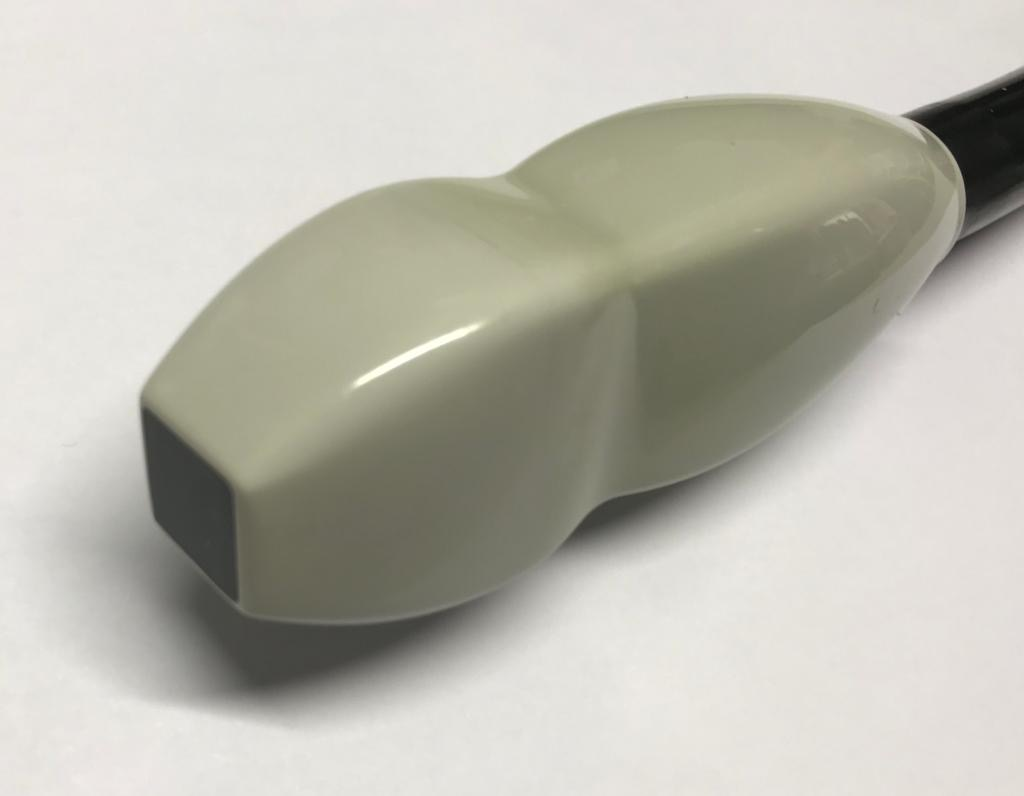
\includegraphics[width = 6cm]{Bilder/transducer.png}
\caption[Transducer]{2D matrix transducer}
\label{fig:transducer}
\end{minipage}
\end{figure}

\newpage
\section{Implementation}
\subsection{Delay and Sum for 3D}
For the implementation of the Delay and Sum beamformer refer to the files in src/SupraLib/Beamformer starting with RxSampleBeamformerDelayAndSum.
The basic idea of this adaption of the existing algorithm is to use the raw data received from the transducer and to perform the beamforming in direction of the X axis and then in the direction of the Y axis.
Both results are then added and returned.
\begin{itemize}
  \item RxSampleBeamformerDelayAndSum.h:

    By using this implementation, the algorithm is designed to iterate along the X axis and for each element to iterate over the Y axis.
    For the summation of the values, the weights of the corresponding elements are considered.
    In general, the file has remained unchanged during the implementation of the beamformers.

    The implementation provides two methods, one for the beamforming in 2D and one for 3D.
      \begin{itemize}
        \item sampleBeamform2D():
          This method performs the Delay and Sum beamforming algorithm for 2D.
          This file has remained unchanged during the implementation of the changes of the 3D beamformer.
        \item sampleBeamform3D():
          This method performs the Delay and Sum beamforming algorithm for 3D.
          This file has remained unchanged during the implementation of the changes of the 3D beamformer.
          The algorithm is designed to iterate over the X axis.
          During this iteration, the values along the Y axis are summed up (multiplied with the corresponding weights).
      \end{itemize}

  \item RxSampleBeamformerDelayAndSumYX.h:

    By using this implementation, the algorithm is designed like the algorithm of the beamformer above, just swapping the X and Y axis.
    The algorithm iterates along the Y axis and for each element it iterates over the X axis.
    For the summation of the values the weights of the corresponding elements are considered.

    The implementation provides two methods, one for the beamforming in 2D and one for 3D.
      \begin{itemize}
        \item sampleBeamform2D():
          Same function as sampleBeamform2D() in the class RxSampleBeamformerDelayAndSum.
        \item sampleBeamform3D():
          This method performs the Delay and Sum beamforming algorithm for 3D.
          Therefore, it call the function sampleBeamform3DYX() with the corresponding arguments.
        \item sampleBeamform3DYX():
          The algorithm is designed to iterate over the Y axis.
          During this iteration, the values along the X axis are summed up (multiplied with the corresponding weights).
          This method is called by sampleBeamform3D().
      \end{itemize}

  \item RxSampleBeamformerDelayAndSumXYYX.h:

    By using this implementation, the algorithm unifies both algorithms from the two beamformers above.
    Again, for the summation of the values the weights of the corresponding elements are considered.

    The implementation provides two methods, one for the beamforming in 2D and one for 3D.
      \begin{itemize}
        \item sampleBeamform2D():
          Same function as sampleBeamform2D() in the class RxSampleBeamformerDelayAndSum.
        \item sampleBeamform3D():
          This method performs the Delay and Sum beamforming algorithm for 3D.
          Therefore, it call the function sampleBeamform3DXY() with the corresponding arguments, as well as the function sampleBeamform3DYX() with the corresponding arguments.
          The results are added and returned.
        \item sampleBeamform3DXY():
          The algorithm is designed to iterate over the X axis.
          During this iteration, the values along the Y axis are summed up (multiplied with the corresponding weights).
        \item sampleBeamform3DYX():
          The algorithm is designed to iterate over the Y axis.
          During this iteration, the values along the X axis are summed up (multiplied with the corresponding weights).
      \end{itemize}

  \item RxSampleBeamformerDelayAndSumXYYXDivided.h:

    By using this implementation, the algorithm unifies the both algorithms from the two beamformers above and halves the result before returning.
    Again, for the summation of the values the weights of the corresponding elements are considered.

    The implementation provides two methods, one for the beamforming in 2D and one for 3D.
      \begin{itemize}
        \item sampleBeamform2D():
          Same function as sampleBeamform2D() in the class RxSampleBeamformerDelayAndSum.
        \item sampleBeamform3D():
          This method performs the Delay and Sum beamforming algorithm for 3D.
          Therefore, it call the function sampleBeamform3DXY() with the corresponding arguments, as well as the function sampleBeamform3DYX() with the corresponding arguments.
          The results are added, divided by two and returned.
        \item sampleBeamform3DXY():
          The algorithm is designed to iterate over the X axis.
          During this iteration, the values along the Y axis are summed up (multiplied with the corresponding weights).
        \item sampleBeamform3DYX():
          The algorithm is designed to iterate over the Y axis.
          During this iteration, the values along the X axis are summed up (multiplied with the corresponding weights).
      \end{itemize}
\end{itemize}

\subsection{Delay Multiply and Sum}
For the implementation of the Delay Multiply and Sum beamformer (according to \cite{articleAboutSDMAS}) refer to the files in src/SupraLib/Beamformer starting with RxSampleBeamformerDelayMultiplyAndSum.

\begin{itemize}
  \item RxSampleBeamformerDelayMultiplyAndSum.h:

    The implementation provides two methods, one for the beamforming in 2D and one for 3D.
      \begin{itemize}
        \item sampleBeamform2D():
          Implementation of the 2D DMAS beamformer considering the weights of the elements, as well as the normalization of the result with the number of accumulated elements and multiplied with the accumulated weights of the elements.
          For performing the beamforming, the algorithm iterates over the receiving window choosing one index as the active element.
          For this active element each of the remaining elements on its right side are multiplied with the value of the active element and the corresponding weights and then summed up.
          For the accumulated weight, the product of both the weight of the actual element and the element, which is iterated over, is summed up.
          In general, the method refers to the elements of the element, being iterated over, with the name affix 'Shift'.
        \item sampleBeamform3D():
          Implementation of the 3D DMAS beamformer, adapted from the 2D DMAS beamformer, considering the weights of the elements, as well as the normalization of the result with the number of accumulated elements and multiplied with the accumulated weights of the elements.
          The algorithm is designed to iterate over the receiving window.
          Therefore, the algorithm picks an active element for which an subwindow is chosen, starting with at the next column and next row of the receiving window.
          Again, the value of active element, the element, which is iterated over and the corresponding weights are multiplies and summed.
          In general, the method refers to the elements of the element, being iterated over, with the name affix 'Shift'.
      \end{itemize}

  \item RxSampleBeamformerDelayMultiplyAndSum2.h:

    The implementation provides just one usable method, the one for the beamforming in 2D.
      \begin{itemize}
        \item sampleBeamform2D():
          Implementation of the 2D DMAS beamformer considering the weights of the elements, but without the normalization of the result with the number of accumulated elements and multiplied with the accumulated weights of the elements.
          For performing the beamforming, the algorithm iterates over the receiving window choosing one index as the active element.
          For this active element each of the remaining elements on its right side are multiplied with the value of the active element and the corresponding weights and then summed up.
          For the accumulated weight, the product of both the weight of the actual element and the element, which is iterated over, is summed up.
          In general, the method refers to the elements of the element, being iterated over, with the name affix 'Shift'.
        \item sampleBeamform3D():
          Not implemented - use RxSampleBeamformerDelayMultiplyAndSum.
      \end{itemize}

  \item RxSampleBeamformerDelayMultiplyAndSum3.h:

    The implementation provides just one usable method, the one for the beamforming in 2D.
      \begin{itemize}
        \item sampleBeamform2D():
          Implementation of the 2D DMAS beamformer considering the weights of the elements, as well as the normalization of the result with the number of accumulated elements and multiplied with the accumulated weights of the elements.
          For performing the beamforming, the algorithm iterates over the receiving window choosing one index as the active element.
          For this active element each of the remaining elements on its right side are multiplied with the value of the active element and then summed up.
          For the accumulated weight, the product of both the weight of the actual element and the element, which is iterated over, is summed up.
          The difference is, that for the summation of the multiplied values the weights are not considered.
          In general, the method refers to the elements of the element, being iterated over, with the name affix 'Shift'.
        \item sampleBeamform3D():
          Not implemented - use RxSampleBeamformerDelayMultiplyAndSum.
      \end{itemize}

  \item RxSampleBeamformerDelayMultiplyAndSum4.h:

    The implementation provides just one usable method, the one for the beamforming in 2D.
      \begin{itemize}
        \item sampleBeamform2D():
          Implementation of the 2D DMAS beamformer.
          For performing the beamforming, the algorithm iterates over the receiving window choosing one index as the active element.
          For this active element each of the remaining elements on its right side are multiplied with the value of the active element and then summed up.
          In this algorithm, neither weights are considered, nor normalization is performed.
          In general, the method refers to the elements of the element, being iterated over, with the name affix 'Shift'.
        \item sampleBeamform3D():
          Not implemented - use RxSampleBeamformerDelayMultiplyAndSum.
      \end{itemize}
\end{itemize}

\subsection{Signed Delay Multiply and Sum}
For the implementation of the Delay Multiply and Sum beamformer (according to \cite{articleAboutSDMAS}) refer to the header file src/SupraLib/Beamformer/RxSampleBeamformerSignedDelayMultiplyAndSum.h

\begin{itemize}
  \item RxSampleBeamformerSignedDelayMultiplyAndSum.h:

    The implementation provides just one usable method, the one for the beamforming in 2D.
      \begin{itemize}
        \item sampleBeamform2D():
          Implementation of the 2D SDMAS beamformer.
          For performing the beamforming, the algorithm returns the result of the Delay Multiply and Sum beamformer with the same sign as the result of the Delay and Sum beamformer would have.
        \item sampleBeamform3D():
          Not implemented - use RxSampleBeamformerDelayMultiplyAndSum.
      \end{itemize}

\end{itemize}

\bibliography{literatur}

\end{document}
